% !TeX encoding = windows-1251
\documentclass[12pt,a4paper]{article}
\usepackage[mag=1000]{newlistok}

\УвеличитьШирину{1cm}
\УвеличитьВысоту{2.1cm}
%\renewcommand{\spacer}{\vspace{2pt}}

\ВключитьКолонтитул


\begin{document}

\Заголовок{Принцип Дирихле: задачи посложнее}
\НадНомеромЛистка{179 школа, 7Б.}
\НомерЛистка{3}
\ДатаЛистка{09.2017}
\СоздатьЗаголовок

%\smallskip

\раздел{Примеры задач с решениями}

\пример\em
Докажите, что в любой компании из 5 человек есть двое, имеющие одинаковое число знакомых в этой компании.
\кпример
\решение
Предположим противное --- у всех разное число знакомых. Заметим, что у каждого человека в этой компании может быть 0, 1, 2, 3 или 4 знакомых, всего 5 вариантов. Но и человек всего 5, а значит, все эти варианты присутствуют.
Но в компании не могут одновременно находиться человек, знакомый со всеми, и человек, незнакомый ни с кем. Противоречие.
\крешение
%Поэтому остаются 4 варианта
%Если у некоторого человека А имеется 4 знакомых, то каждый в компании знаком с человеком А, и не может быть человека, имеющего 0 знакомых. Значит в компании либо не будет человека, имеющего 4 знакомых, либо не будет человека, имеющего 0 знакомых. Имеем 5 человек и 4 варианта возможных количеств знакомых (либо 0, 1, 2, 3, либо 1, 2, 3, 4). Тогда по принципу Дирихле найдутся два человека, имеющие одинаковое число знакомых в этой компании.

\пример\em
Дано 52 различных натуральных числа, не превосходящих 100. Докажите, что из них всегда можно выбрать два, одно из которых на три больше другого.
\кпример
\решение
 Разобьём первые 100 натуральных чисел на три такие последовательности:\\
%, в первой из которых 34, а в двух других по 33 числа:\\
\hspace*{8cm}$1,4, 7,10,..., 97, 100;$\\
\hspace*{8cm}$2,	5, 8,11,..., 98;$\\
\hspace*{8cm}$3,	6, 9,12,..., 99.$

\noindent
В первой 34 числа, в двух других --- по 33, и в каждой последовательности любые два соседних числа отличаются на 3. Докажем, что какие-то два из данных 52 чисел стоят рядом в одной из последовательностей. Разобьем числа в каждой последовательности на группы из двух соседних чисел. В первой последовательности получится 17 пар, во второй и третьей --- по 16 пар и по одному непарному числу. Всего получим $17+16+1+16+1=51$ группу. Поскольку чисел 52, а групп 51, то какие-то два из данных чисел попадут в одну группу. Но числа одной группы различаются на 3, а значит, среди данных 52 чисел есть два, отличающиеся на 3.
\крешение

\раздел{Задачи}

\задача Докажите, что у любого многогранника найдутся две грани с одинаковым числом сторон.
\кзадача

\задача В канун Нового года 10 друзей посылали праздничные открытки друг другу. Каждый послал 5 открыток. Докажите, что найдутся двое, пославшие открытки друг другу.
\кзадача

\задача  На большую «шахматную» доску $2017\times 2017$ поставили 2017 ладей так, что ни одна из них не бьет другую. Докажите, что в любом квадрате
$1009 \times 1009$ найдётся хотя бы одна ладья.
\кзадача

\задача  Петя пытается занумеровать вершины куба числами от 1 до 8 (без повторений) так, чтобы суммы чисел на концах каждого ребра куба были различны. Удастся ли ему это сделать?
\кзадача

\задача  На шахматной доске стоят фигуры: на каждой горизонтали есть хотя бы одна фигура, а на разных горизонталях стоит разное число фигур. Докажите, что можно убрать часть фигур так, что на каждой вертикали и каждой горизонтали останется ровно одна фигура.
\кзадача

\задача В поход пошло 30 школьников. Оказалось, что среди любых 10 из них обязательно найдётся трое одноклассников. Докажите, что в походе приняло участие не менее 8 человек из одного класса.
\кзадача

\задача  Докажите, что из 51 натурального числа первой сотни можно выбрать 6 так, что никакие два из них не имеют одинаковых цифр в одном разряде.
\кзадача

\задача Верно ли, что среди любых \пункт 34; \пункт 32 различных натуральных чисел, не превосходящих 50, всегда можно выбрать два, одно из которых вдвое больше другого?
\кзадача

\задача Даны 70 различных натуральных чисел, каждое из которых не превосходит 200. Докажите, что какие-то два из них отличаются на 4, 5 или 9.
\кзадача


\ЛичныйКондуит{0mm}{6mm}
\ОбнулитьКондуит



\задача  Даны 50 различных натуральных чисел, 25 из которых не больше 50, а остальные больше 50, но не больше 100. При этом никакие два из них не отличаются ровно на 50. Найдите сумму этих чисел.
\кзадача


\задача  Из ряда 1, 2,..., 200 выбрали 101 число. Докажите, что одно из выбранных чисел делится на другое.
\кзадача

\задача  Числа 1, 2, \ldots, 600 выписаны в строчку в неком порядке. Сумма любых двух соседних чисел не больше 800. Докажите, что сумма каких-то двух чисел, идущих через одно, больше 800.
\кзадача



\задача На пир собралось 100 людоедов. Известно, что среди любых 10 хотя бы один оказался в желудке у другого (из этой десятки). Докажите, что есть «матрёшка» из 12 людоедов, каждый из которых (кроме последнего) находится в желудке у следующего.
\кзадача

\задача Пять школьников решили в воскресенье посмотреть все новые фильмы последнего месяца. Для этого был выбран семизальный кинотеатр, в котором сеансы начинаются в 9.00, 10.40, 12.20, 14.00, 15.40, 17.20, 19.00, 20.40 и 22.00. На каждый сеанс школьники делились на две группы, одна шла в один зал, а другая --- в другой. Вечером выяснилось, что каждый школьник побывал в каждом зале. Докажите, что в каждом из залов был сеанс, на котором никто из школьников не был.
\кзадача

\задача В течение прошлого учебного года Саша каждый день решал хотя бы одну задачу по математике. Однако, боясь перетрудиться, за неделю он решал не более 12 задач. Докажите, что можно найти несколько последовательных дней, в течение которых Саша решил ровно 20 задач.
\кзадача

\задача В банде 50 гангстеров. Все вместе они ни в одной разборке ни разу не участвовали, а каждые двое встречались на разборках ровно по разу. Докажите, что кто-то из гангстеров был не менее, чем на восьми разборках.
\кзадача

\задача В каждом из двух одинаковых правильных 16-угольников отметили по 7 вершин. Докажите, что можно так наложить эти многоугольники друг на друга, чтобы не менее 4 отмеченных вершин одного многоугольника совпали с отмеченными вершинами другого.
\кзадача

\задача
Доска $6\times6$ разбита на доминошки. Докажите, что можно разрезать доску по прямой на две части, не повредив ни одной доминошки.
\кзадача

\задача
\пункт Докажите, что если в $3n$ клетках таблицы $2n\times 2n$ расставлены $3n$ звёздочек, то можно вычеркнуть $n$ столбцов и $n$ строк
так, что все звёздочки будут вычеркнуты.\\
\пункт Докажите, что в таблице $2n\times2n$ можно расставить $3n+1$ звёздочек, так что при вычёркивании любых $n$ строк и любых $n$ столбцов остаётся невычеркнутой хотя бы одна звёздочка.
\кзадача

\ЛичныйКондуит{0mm}{6mm}

% \GenXMLW

\end{document}

\newpage

{\bf Старая версия}


{\footnotesize \textbf{Принцип Дирихле.} Пусть есть $n$ ящиков и $n+1$ кроликов. Если расселить кроликов по ящикам, то найдется хотя бы один ящик, в котором
 окажутся не менее $2$ кроликов.}

\задача В мешке имеется $32$ красных шара, $29$ зеленых шаров, $45$ синих, $17$ желтых и по $30$ белых, черных и
серых (всего $213$ шаров). Сколько шаров необходимо вынуть из мешка, чтобы среди них гарантированно
нашлось $9$ шаров одного цвета? \кзадача

\задача Комиссия из $60$ человек провела $40$ заседаний, причем на каждом заседании присутствовали ровно $10$
членов комиссии. Докажите, что найдутся два члена комиссии, по крайней мере дважды встречавшиеся
на заседаниях. \\
{\tt Есть два решения: одно использует комбинаторику (для расчёта количества пар), другое не использует.}
 \кзадача

\задача
В таблице $10 \times 10$ расставлены \пункт числа от 1 до 100; \пункт произвольные целые числа, причем любые два числа в соседних клетках отличаются не более, чем на $5$. Докажите, что среди этих чисел найдутся два равных.
{\tt Это, конечно скорее задача на принцип крайнего, чем на принцип Дирихле}
\кзадача

\задача На шахматной доске стоит 44 ферзя. Докажите, что каждый из них бьёт какого-нибудь другого ферзя.
\кзадача

\задача В клетках таблицы $4 \times 4$ расставлено $6$ звёздочек. Докажите, что из таблицы можно вычеркнуть две строки и два столбца так, что в оставшейся таблице звёздочек не будет.
\кзадача

\задача Клетки доски $8 \times 8$ раскрашены в разные цвета. Назовём клетку {\it счастливой}, если хотя бы две соседние с ней по стороне клетки покрашены в тот же цвет. При каком наибольшем количестве цветов можно раскрасить доску так, что все клетки будут счастливыми?
\кзадача

\сзадача Восемь школьников решали 8 задач. Оказалось, что каждую задачу решили 5 школьников.
Докажите, что найдутся такие два школьника, что каждую задачу решил хотя бы один из них.
{\tt Опять используется комбинаторика. }
\кзадача



% \GenXMLW

\end{document}





































\putthere{169mm}{-11mm}{%
    %
    % пирамидка
      \begin{tikzpicture}
      [scale=.7
    % эти константы задают раскраску граней
      ,fil1/.style={draw=blue!5!black,fill=gray!00,thin}
      ,fil2/.style={draw=blue!5!black,fill=gray!30,thin}
      ,fil3/.style={draw=blue!5!black,fill=gray!69,thin}
      ]
    % эти константы задают наклон кубика
        \coordinate (d) at (50:.6);

        \coordinate (A) at (0,0);
        \coordinate (md) at ($ (0,0) - (d) $);
        \filldraw[fil2] (A) -- +(1,0) -- +(1,1) -- +(0,1) -- cycle;
        \filldraw[fil1] (A)++(1,1) -- ++(d) -- ++(-1,0) -- ++(md) -- cycle;
        \filldraw[fil3] (A)++(1,1) -- ++(d) -- ++(0,-1) -- ++(md) -- cycle;
        \coordinate (A) at ($(0,-1)+(md)$);
        \filldraw[fil2] (A) -- +(1,0) -- +(1,1) -- +(0,1) -- cycle;
        \filldraw[fil1] (A)++(1,1) -- ++(d) -- ++(-1,0) -- ++(md) -- cycle;
        \filldraw[fil3] (A)++(1,1) -- ++(d) -- ++(0,-1) -- ++(md) -- cycle;
        \coordinate (A) at (1,-1);
        \filldraw[fil2] (A) -- +(1,0) -- +(1,1) -- +(0,1) -- cycle;
        \filldraw[fil1] (A)++(1,1) -- ++(d) -- ++(-1,0) -- ++(md) -- cycle;
        \filldraw[fil3] (A)++(1,1) -- ++(d) -- ++(0,-1) -- ++(md) -- cycle;
        \coordinate (A) at ($(1,-1)+(md)$);
        \filldraw[fil2] (A) -- +(1,0) -- +(1,1) -- +(0,1) -- cycle;
        \filldraw[fil1] (A)++(1,1) -- ++(d) -- ++(-1,0) -- ++(md) -- cycle;
        \filldraw[fil3] (A)++(1,1) -- ++(d) -- ++(0,-1) -- ++(md) -- cycle;
       \end{tikzpicture}
}{5cm}{\risn Пирамида для $1^2+2^2$}
\vspace{-4mm}
\УстановитьГраницы{0truecm}{4truecm}


\сзадача Число $k^2$ можно представлять себе как объём параллелепипеда
$1\times k\times k$, а~сумму $1^2+2^2+\ldots+n^2$ --- как объём пирамиды,
сложенной из таких параллелепипедов. Будем обозначать эту пирамиду $Sq(n)$
(на рисунке 3 изображена пирамида $Sq(2)$ объёмом $1^2+2^2$).
Сложите из шести пирамид $Sq(n)$ параллелепипед.
Каковы его размеры и объём? Выведите
формулу для суммы $1^2+2^2+\ldots+n^2$.
\кзадача




\putthere{165mm}{-17mm}{%
    %
    % пирамидки
      \begin{tikzpicture}
      [scale=.35
      ,fil1/.style={draw=blue!5!black,fill=gray!00,thin}
      ,fil2/.style={draw=blue!5!black,fill=gray!30,thin}
      ,fil3/.style={draw=blue!5!black,fill=gray!69,thin}
      ]
        \coordinate (d) at (50:.6);
        \coordinate (A1) at (0,0);
        \coordinate (A2) at (5,0);
        \coordinate (A3) at (10,0);
        \coordinate (md) at ($ (0,0) - (d) $);

        \foreach \x/\y/\z in {1/4/3, 1/4/4, 2/3/2, 1/3/3, 2/3/3, 3/2/1, 1/2/2, 2/2/2, 3/2/2, 1/1/1, 2/1/1, 3/1/1, 4/1/1}
        {
            \coordinate (A) at ($ (A1) + \x*(1,0) + \z*(0,1) + \y*(d)$);
            \filldraw[fil2] (A) -- +(1,0) -- +(1,1) -- +(0,1) -- cycle;
            \filldraw[fil1] (A)++(1,1) -- ++(d) -- ++(-1,0) -- ++(md) -- cycle;
            \filldraw[fil3] (A)++(1,1) -- ++(d) -- ++(0,-1) -- ++(md) -- cycle;
        }

        \foreach \x/\y/\z in {1/4/1, 1/4/2, 1/4/3, 1/4/4, 2/4/3, 2/3/1, 2/3/2, 2/3/3,   3/4/2, 3/3/2, 3/2/1, 3/2/2,  4/4/1, 4/3/1, 4/2/1, 4/1/1}
        {
            \coordinate (A) at ($ (A2) + \x*(1,0) + \z*(0,1) + \y*(d)$);
            \filldraw[fil2] (A) -- +(1,0) -- +(1,1) -- +(0,1) -- cycle;
            \filldraw[fil1] (A)++(1,1) -- ++(d) -- ++(-1,0) -- ++(md) -- cycle;
            \filldraw[fil3] (A)++(1,1) -- ++(d) -- ++(0,-1) -- ++(md) -- cycle;
        }

        \foreach \x/\y/\z in {4/4/1, 4/3/1, 4/2/1, 4/1/1, 1/4/4, 4/4/2, 4/3/2, 4/2/2, 2/4/4, 3/4/4, 4/4/3, 4/4/4,  2/3/3, 3/3/3, 4/3/3, 3/2/2, 4/2/2}
        {
            \coordinate (A) at ($ (A3) + \x*(1,0) + \z*(0,1) + \y*(d)$);
            \filldraw[fil2] (A) -- +(1,0) -- +(1,1) -- +(0,1) -- cycle;
            \filldraw[fil1] (A)++(1,1) -- ++(d) -- ++(-1,0) -- ++(md) -- cycle;
            \filldraw[fil3] (A)++(1,1) -- ++(d) -- ++(0,-1) -- ++(md) -- cycle;
        }

       \end{tikzpicture}
}{5cm}{\risn Интересные пирамиды}
\vspace{-4mm}
\УстановитьГраницы{0truecm}{6.4truecm}


\задача
\putthere{160mm}{-70mm}{%
    %
    % Таблица
    %
      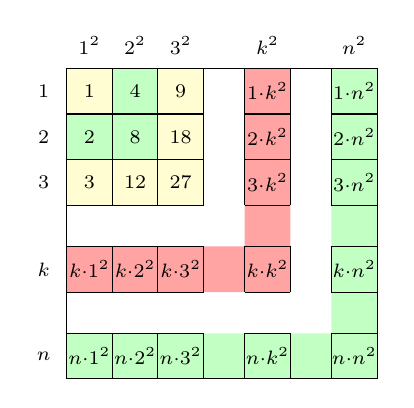
\begin{tikzpicture}
      [scale=.58
      ,fil1/.style={color=green!40!white,opacity=.6}
      ,fil2/.style={color=red!60!white,opacity=.6}
      ,fil3/.style={color=yellow!30!white,opacity=.6}
      ,lin/.style={color=black!100}
      ]
        \fill[fil1] (6.3,-0.5) -- (7.3,-0.5) -- (7.3, -7.3) -- (0.5,-7.3) -- (0.5,-6.3) -- (6.3,-6.3) -- cycle;
        \fill[fil2] (4.4,-0.5) -- (5.4,-0.5) -- (5.4, -5.4) -- (0.5,-5.4) -- (0.5,-4.4) -- (4.4,-4.4) -- cycle;
        \fill[fil3] (2.5,-0.5) -- (3.5,-0.5) -- (3.5, -3.5) -- (0.5,-3.5) -- (0.5,-2.5) -- (2.5,-2.5) -- cycle;
        \fill[fil1] (1.5,-0.5) -- (2.5,-0.5) -- (2.5, -2.5) -- (0.5,-2.5) -- (0.5,-1.5) -- (1.5,-1.5) -- cycle;
        \fill[fil3] (0.5,-0.5) -- (1.5,-0.5) -- (1.5, -1.5) -- (0.5,-1.5) -- cycle;
        \foreach \i in {1.5, 2.5, 3.5, 4.4, 5.4,  6.3}{
          \draw[lin] (0.5, -\i) -- (3.5, -\i);
          \draw[lin] (4.4, -\i) -- (5.4, -\i);
          \draw[lin] (6.3, -\i) -- (7.3, -\i);
          \draw[lin] (\i, -0.5) -- (\i, -3.5);
          \draw[lin] (\i, -4.4) -- (\i, -5.4);
          \draw[lin] (\i, -6.3) -- (\i, -7.3);
        }
        \draw[lin] (0.5, -0.5) -- (0.5, -7.3);
        \draw[lin] (0.5, -0.5) -- (7.3, -0.5);
        \draw[lin] (7.3, -7.3) -- (0.5, -7.3);
        \draw[lin] (7.3, -7.3) -- (7.3, -0.5);
        \draw (1, -1) node {$\scriptstyle 1$};
        \draw (2, -1) node {$\scriptstyle 4$};
        \draw (3, -1) node {$\scriptstyle 9$};
        \draw (1, -2) node {$\scriptstyle 2$};
        \draw (2, -2) node {$\scriptstyle 8$};
        \draw (3, -2) node {$\scriptstyle 18$};
        \draw (1, -3) node {$\scriptstyle 3$};
        \draw (2, -3) node {$\scriptstyle 12$};
        \draw (3, -3) node {$\scriptstyle 27$};
        \foreach \i in {1,2,3}
        {
          \draw (\i, -4.9) node {$\scriptstyle k\cdot\i^2$};
          \draw (4.9, -\i) node {$\scriptstyle\i\cdot k^2$};
          \draw (\i, -6.8) node {$\scriptstyle n\cdot\i^2$};
          \draw (6.8, -\i) node {$\scriptstyle\i\cdot n^2$};
          \draw (\i, 0) node {$\scriptstyle \i^2$};
          \draw (0, -\i) node {$\scriptstyle \i$};
        }

        \draw (4.9, -4.9) node {$\scriptstyle k\cdot k^2$};
        \draw (6.8, -4.9) node {$\scriptstyle k\cdot n^2$};
        \draw (4.9, -6.8) node {$\scriptstyle n\cdot k^2$};
        \draw (6.8, -6.8) node {$\scriptstyle n\cdot n^2$};
        \draw (4.9, 0) node {$\scriptstyle k^2$};
        \draw (6.8, 0) node {$\scriptstyle n^2$};
        \draw (0, -4.9) node {$\scriptstyle k$};
        \draw (0, -6.8) node {$\scriptstyle n$};

      \end{tikzpicture}
}{7cm}{}%{\risn Таблица умножения\\чисел и их квадратов}
На рисунке справа изображены несколько пирамид высоты~4,
каждая из них состоит из $T_1+T_2+T_3+T_4$ кубиков.
\пункт Выберите одну из пирамид на рисунке и нарисуйте её горизонтальные слои:
нижний, второй снизу, \dots , верхний.
\пункт Нарисуйте передний, второй спереди, \dots ,
задний слои выбранной пирамиды;
\пункт Нарисуйте самый левый, второй слева, \dots, самый правый слои выбранной пирамиды.
\пункт Сложите из шести пирамид такого вида параллелепипед. Каковы его размеры?
\ВосстановитьГраницы
\noindent\hspace*{-3.5mm}\пункт Как сложить параллелепипед из шести пирамид аналогичного вида,
но высоты $n$? Найдите формулу для суммы треугольных чисел $T_1+T_2+\dots+T_n$
(эта сумма обозначается $П_n$ и
называется {\it $n$-ым пирамидальным числом}).
\пункт
Сложите из двух таких пирамид высоты $n$ и высоты $n-1$
пирамиду $Sq(n)$ и выведите формулу
для суммы $1^2+2^2+\ldots+n^2$.
\пункт Докажите геометрически, что\\
\noindent%
$T_1+T_2+\dots+T_n=
1\cdot n+2\cdot(n-1)+3\cdot(n-2)+\dots+(n-1)\cdot2+n\cdot1$.
\кзадача

\УстановитьГраницы{0mm}{45mm}
\сзадача Найдите сумму квадратов первых $n$ нечётных чисел. \кзадача

\сзадача
%Придумайте какой-нибудь способ получения формул для следующих сумм
Найдите (каким-нибудь способом) формулу для суммы
%(геометрическое решение составителям неизвестно):
%\вСтрочку
%\пункт
$П_1+П_2+\ldots+П_n$. %;
%\пункт $1^4+2^4+\ldots+n^4$.
\кзадача

\сзадача
На рисунке справа изображена таблица умножения чисел
$1$, $2$, \dots , $n$ на числа $1^2$, $2^2$, \dots, $n^2$.
\пункт Найдите сумму всех чисел в этой таблице.
\пункт Найдите сумму чисел, стоящих в выделенном уголке
(представьте в виде многочлена от $k$).
\пункт Выведите формулу для суммы $1^4+2^4+\ldots+n^4$.
\кзадача

%\сзадача
%Придумайте какой-нибудь способ получения формул для следующих сумм
%(геометрическое решение составителям неизвестно):
%\вСтрочку
%\пункт $П_1+П_2+\ldots+П_n$;
%\пункт $1^4+2^4+\ldots+n^4$.
%\кзадача

\vspace{1mm}
Интересно, какие ещё суммы можно найти с помощью геометрических рассуждений?


\putthere{163mm}{-13mm}{%
    %
    % Картинка для пятиугольных чисел
      \begin{tikzpicture}
      [scale=.11
      ,ver/.style={circle,draw=blue!50,fill=blue!20,thick,inner sep=0,minimum size=3}
      ,lin/.style={color=blue!80}]
        \coordinate (A0) at (0,0);
        \coordinate (A1) at (7,0);
        \coordinate (A2) at (20,0);
        \coordinate (A3) at (42,0);
        \node[ver] at (A0){};
        \draw[lin,very thin] (A1) + (-126:4) -- +(18:4);
        \draw[lin,very thin] (A1) + (-126:4) -- +(90:4);
        \foreach \a in {18,90,...,306}{
          \draw[lin] (A1)
                                       +(\a:4)    node[ver]{}
                                    -- +(\a+72:4);
        }
        \draw[lin,very thin] (A2) + (-126:8) -- +(18:8);
        \draw[lin,very thin] (A2) + (-126:8) -- +(90:8);
        \foreach \a in {18,90,...,306}{
          \draw[lin] (A2)
                                       +(\a:8)    node[ver]{} coordinate (A)
                                    -- +(\a+72:8)             coordinate (B);
          \node[ver] at  ($ (A)!.5!(B) $){};
          \draw[lin] (A2) ++ (-126:8) ++ (54:4)
                                       +(\a:4)    node[ver]{} coordinate (A)
                                    -- +(\a+72:4)             coordinate (B);
        }
        \draw[lin,very thin] (A3) + (-126:12) -- +(18:12);
        \draw[lin,very thin] (A3) + (-126:12) -- +(90:12);
        \foreach \a in {18,90,...,306}{
          \draw[lin] (A3)
                                       +(\a:12)    node[ver]{} coordinate (A)
                                    -- +(\a+72:12)             coordinate (B);
          \node[ver] at  ($ (A)!.333!(B) $){};
          \node[ver] at  ($ (A)!.666!(B) $){};
          \draw[lin] (A3) ++ (-126:12) ++ (54:8)
                                       +(\a:8)    node[ver]{} coordinate (A)
                                    -- +(\a+72:8)             coordinate (B);
          \node[ver] at  ($ (A)!.5!(B) $){};
          \draw[lin] (A3) ++ (-126:12) ++ (54:4)
                                       +(\a:4)    node[ver]{} coordinate (A)
                                    -- +(\a+72:4)             coordinate (B);
        }
      \end{tikzpicture}
}{7cm}{\risn Пятиугольные числа.}
\vspace{-4mm}
\УстановитьГраницы{0truecm}{6.5truecm}



% \задача
% Сформулируйте и докажите теорему, описывающую явление: \\
% $3+5=2^3$,~$7+9+11=3^3$,~$13+15+17+19=4^3$,~$\ldots$
% \кзадача

\задача
{\it Пятиугольные числа} $P_1=1$, $P_2=5$,
$P_3=12$, $P_4=22$, $\ldots$  показаны на рисунке~2.
Найдите разность $P_k-P_{k-1}$
между последовательными пятиугольными числами.
Выразите $P_n$ через~$n$.
\кзадача

\задача Докажите геометрически, что сумма $n$-го треугольного и $n$-го
четырёхугольного числа на $n$ больше, чем $n$-ое пятиугольное число, .
\кзадача
\ВосстановитьГраницы
